\chapter{THEORETICAL OVERVIEW}
 \label{Chapter 3}
 \lhead{Chapter 3. \emph{Theoretical Overview}}

This chapter provides a theoretical overview of the project as well as specifications for different hardware tools and technologies that are employed.

\section{Hardware Specification}
We use two esp32(ESP-WROOM32) microcontrollers one as a transmitter, and one as a receiver. The features of the device are given below \cite{espDocs}:

\begin{easylist}
 \ListProperties(Style1*=\bfseries,Numbers2=l, Mark1={}, Mark2={)},Indent2=2em)
@ Processors
@@ CPU: Xtensa dual-core (or single-core) 32-bit LX6 microprocessor, operating at 160 or 240 MHz and performing at up to 600 DMIPS
@@ Ultra-low power (ULP) co-processor
@ Memory: 320 KiB RAM, 448 KiB ROM
@ Wireless connectivity:
@@ Wi-Fi: 802.11 b/g/n
@@ Bluetooth: v4.2 BR/EDR and BLE (shares the radio with Wi-Fi)
@ Peripheral interfaces:
@@ 34 × programmable GPIOs
@@ 12-bit SAR ADC up to 18 channels
@@ 2 × 8-bit DACs
@@ 10 × touch sensors (capacitive sensing GPIOs)
@@ 4 × SPI
@@ 2 × I²S interfaces
@@ 2 × I²C interfaces
@@ 3 × UART
@@ SD/SDIO/CE-ATA/MMC/eMMC host controller
@@ SDIO/SPI slave controller
@@ Ethernet MAC interface with dedicated DMA and planned IEEE 1588 Precision Time Protocol support[4]
@@ CAN bus 2.0
@@ Infrared remote controller (TX/RX, up to 8 channels)
@@ Motor PWM
@@ LED PWM (up to 16 channels)
@@ Hall effect sensor
@@ Ultra low power analog preamplifier
@Security:
@@IEEE 802.11 standard security features all supported, including WPA, WPA2, WPA3 (depending on   version)[5] and WLAN Authentication and Privacy Infrastructure (WAPI)
@@     Secure boot
@@     Flash encryption
@@     1024-bit OTP, up to 768-bit for customers
@@     Cryptographic hardware acceleration: AES, SHA-2, RSA, elliptic curve cryptography (ECC), random number generator (RNG)
@Power management:
@@     Internal low-dropout regulator
@@     Individual power domain for RTC
@@     5 $\mu$A deep sleep current
@@     Wake up from GPIO interrupt, timer, ADC measurements, capacitive touch sensor interrupt

\end{easylist}

\begin{figure}[H]
\centering
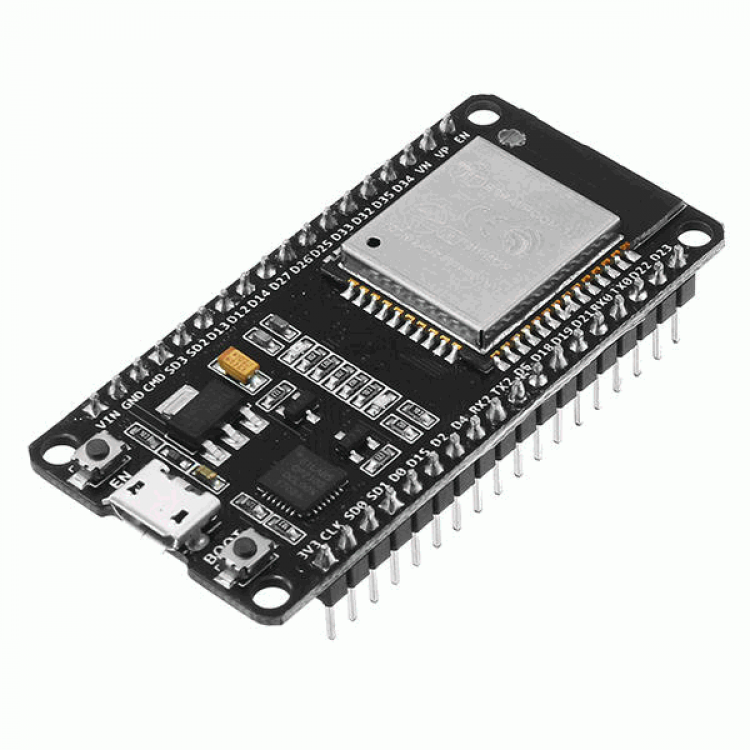
\includegraphics[width=0.7\textwidth]{./figure/chap 3/1.png}
\caption{ A esp32 microcontroller}
\label{Fig 3.1}
\end{figure}

\begin{figure}[H]
\centering
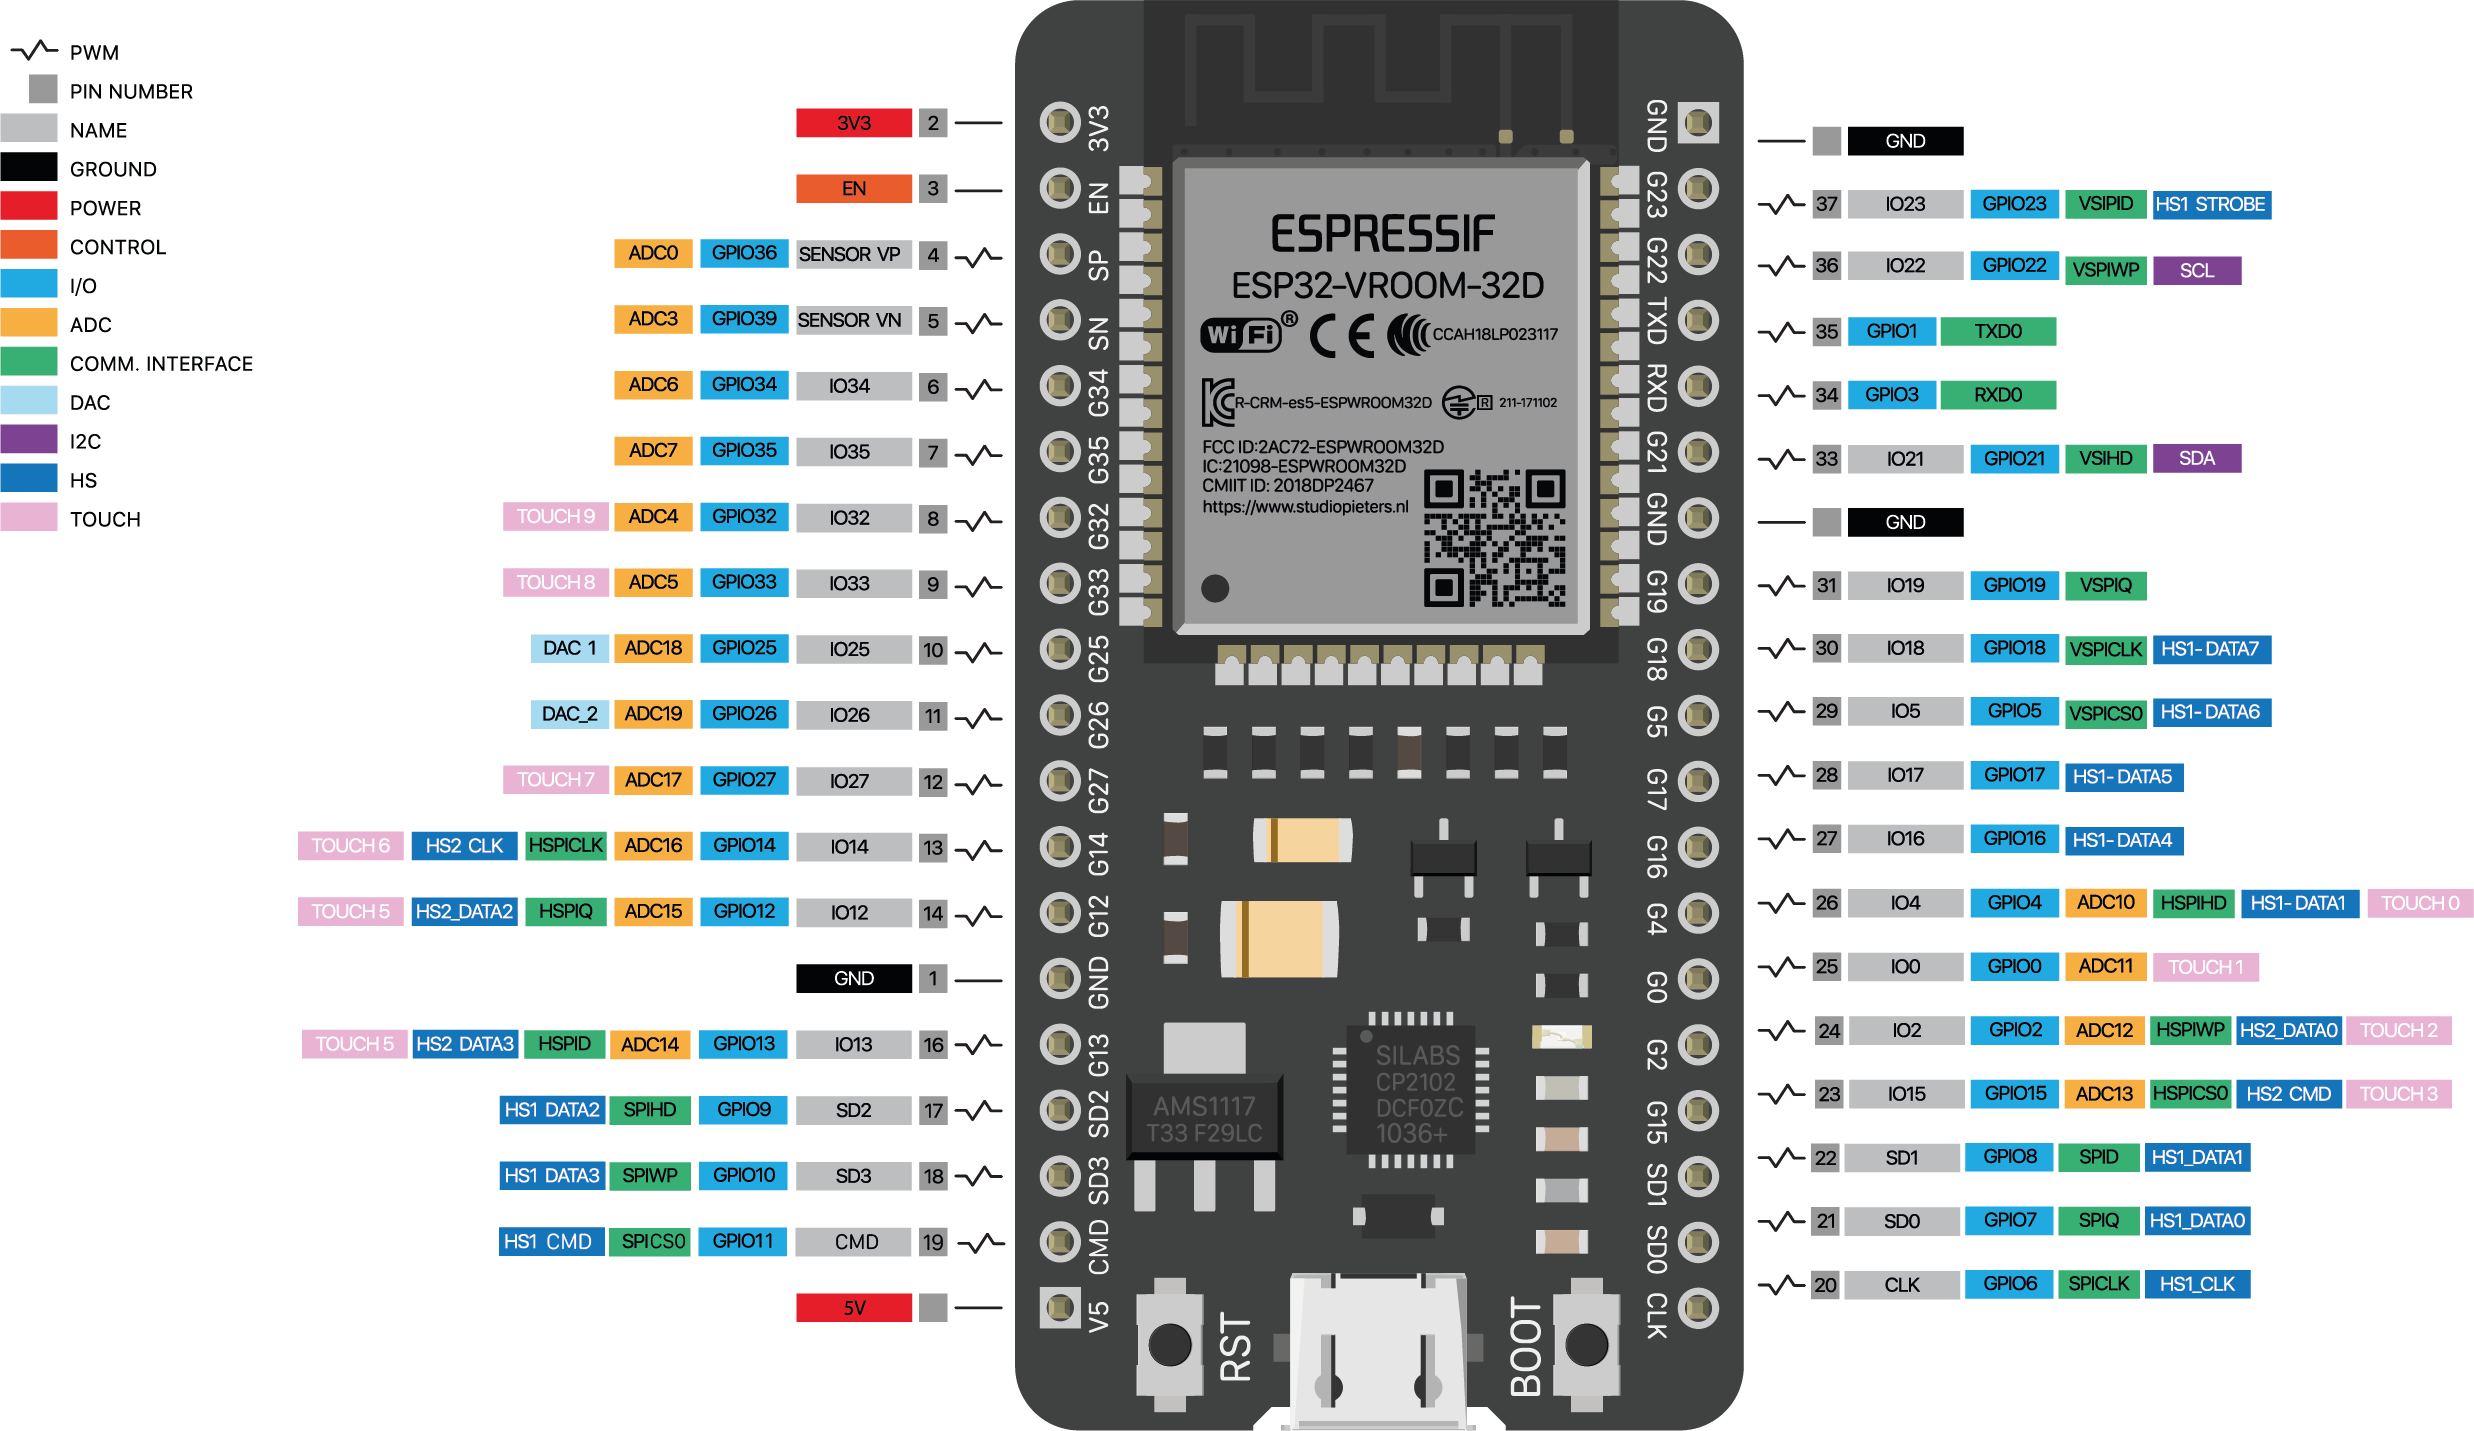
\includegraphics[width=0.7\textwidth]{./figure/chap 3/2.png}
\caption{Pinout diagram of esp32 microcontroller}
\label{Fig 3.2}
\end{figure}

The signal specification for esp32 microconroller is given below:
\begin{itemize}

\item    Bandwidth: 20 MHz
\item    Antenna: 1 RX and 1 TX
\item    Protocol: 802.11n
\item    Modulation: OFDM (16 QAM)
\item    Subcarrier Number:  64
\item    Sampling Rate:  3.9 Hz
\item    Average RSSI: -77 dBm
\item    Guard Interval: 800 ns (MCS Index: 4)
\item    Technologies: MIMO, Frame Aggregation

\end{itemize}

The advantages of using esp32 are:
\begin{itemize}
\item esp32 can function as a stand-alone system or as a slave device to a host MCU, eliminating communication stack overhead on the primary application CPU.
\item Through its SPI / SDIO or I2C / UART interfaces, the esp32 may communicate with other systems to provide Wi-Fi and Bluetooth capability.
\item esp32 has a low-power processor designed for mobile devices, wearable electronics, and IoT applications. It uses a combination of proprietary software to achieve ultra-low power consumption.
\item esp32 is highly-integrated with in-built antenna switches, RF balun, power amplifier, low-noise receive amplifier, filters, and power management modules.
\end{itemize}

In summary, esp32 is ideal for our project because is a power-efficient device that is capable of using wifi communication, is easily integrable with other systems, and has a fair amount of computing power.


\section{Wi-Fi}
In this project, we exploited the capability of Wi-Fi technology to implement fall detection. Wi-Fi, vastly used in high-speed internet access and wireless communication, is a set of protocols governed by IEEE 802.11 standards \cite{7786995}. IEEE 802.11 is part of the local area network (LAN) technical standards and specifies the set of protocols for implementing wireless local area network (WLAN) computer communication. These standards are maintained by the Institute of Electrical and Electronics Engineers (IEEE). Though the first edition of these standards was released in 1997, continuous development is being made and new standards are coming with more capabilities to meet the ever-increasing demand for high-speed wireless communication. The most notable standards of IEEE 802.11 are 802.11a, 802.11b, 802.11g, 802.11n, 802.11ac, and 802.11ax.

\subsection{802.11a}
This was the first standard to use the 5 GHz band for Wi-Fi which might seem to be ahead of its time. But because of the higher frequency, its coverage area was much lower than the traditional 2.4 GHz band and suffered much from interference problem. That is why 802.11a was not so popular compared to its 2.4 GHz counterpart even though it had a higher data rate and went obsolete quickly. But the main contribution of this standard was the introduction of Orthogonal Frequency-Division Multiplexing (OFDM) which improved the data transmission drastically. OFDM is based on the concept of orthogonal subcarriers with minimal interference that makes it possible to cope with severe channel conditions without complex equalization filters. OFDM is described in detail later in this section. 802.11a uses 52 subcarriers in OFDM, of which 48 subcarriers are used for data transmission and the rest 4 subcarriers are used as pilot subcarriers.

\subsection{802.11b}
802.11b was the first widely accepted standard of Wi-Fi. Both 802.11a and 802.11b were released in 1999, with a major difference between them. Unlike 802.11a, 802.11b uses 2.4 GHz band. The 2.4 GHz band was not as crowded as today and offered higher coverage and the capability to withstand interference. These advantages made 802.11b popular despite having a much lower data rate (up to 5.5 Mbit/s). This standard is still in use in some legacy devices.

\subsection{802.11g}
Introduced in 2003, 802.11g was a mixture of the previous two standards. It operated in the 2.4 GHz band like 802.11b and utilizes the same OFDM-based transmission scheme as 802.11a. This technical change gave a burst increase in the data rate which could go up to 54 Mbit/s. 802.11g also uses a total of 52 subcarriers with a carrier separation of 0.3125 MHz. There are 14 partially overlapping channels each of which has a separation of 20 or 25 MHz.

\subsection{802.11n}
This standard is also known as Wi-Fi Generation 4 (Wi-Fi 4). It includes several new technologies that increased the capability of Wi-Fi further. The most notable additions to this standard are:
\begin{itemize}
    \item Multiple Input Multiple Output (MIMO)
    \item Frame aggregation
    \item WiFi Beamforming (Optional)
    \item 40 MHz channel bandwidth
    \item Security enhancement
\end{itemize}
MIMO technology is capable of conducting simultaneous data transmission over multiple antennas. Frame aggregation allows sending two or more frames in a single transmission. Beamforming improves the user experience by focusing the Wi-Fi beams in the user's direction. Thus these new features along with OFDM increased the data rate from 72 Mbit/s to 600 Mvit/s. 802.11n has support for the 2.4 GHz band and optionally for the 5 GHz band. Most Wi-Fi-enabled devices are still using this standard today.

\subsection{Newer standards}
After 802.11n, a few major standards have come out that have increased the data rate, reliability, and security further. 802.11ac (Wi-Fi 5) is currently spreading in the consumer community which uses only the 5 GHz band. It introduced a few new features, such as Multi-User MIMO (MU-MIMO), wider 80 MHz and 160 MHz channels, and Beamforming. 

802.11ax (Wi-Fi 6E) is the most recently approved standard adopted in 202 which uses three bands: 2.4 GHz, 5 GHz, and 6 GHz. The data rate can vary from 600 Mbit/s to 9608 Mbit/s. Currently, the development is being made for 802.11be standard or Wi-Fi 7 which will provide even more data rate.

The hardware used in our proposed method, esp32 uses the popular IEEE 802.11n standard. It currently has the largest user base and can utilize several recent technologies including OFDM, MIMO, and frame aggregation.

\subsection{OFDM}

Orthogonal Frequency-Division Multiplexing (OFDM) is a sort of digital transmission and a way of encoding digital data on multiple carrier frequencies that is used in telecommunications. OFDM is a widely used wideband digital communication technique, with applications including digital television and audio broadcasting, DSL internet access, wireless networks, power line networks, and 4G/5G mobile communications.\cite{1}
The capacity of OFDM to cope with severe channel conditions without the use of sophisticated equalization filters is its fundamental benefit over single-carrier methods. Because OFDM uses numerous slowly modulated narrowband signals rather than a single rapidly modulated wideband signal, channel equalization is simpler. This mechanism also makes it easier to design single frequency networks (SFNs), in which multiple adjacent transmitters send the same signal at the same frequency at the same time, because the signals from multiple distant transmitters can be constructively recombined, avoiding the interference that a traditional single-carrier system would face.

\begin{figure}[H]
\centering
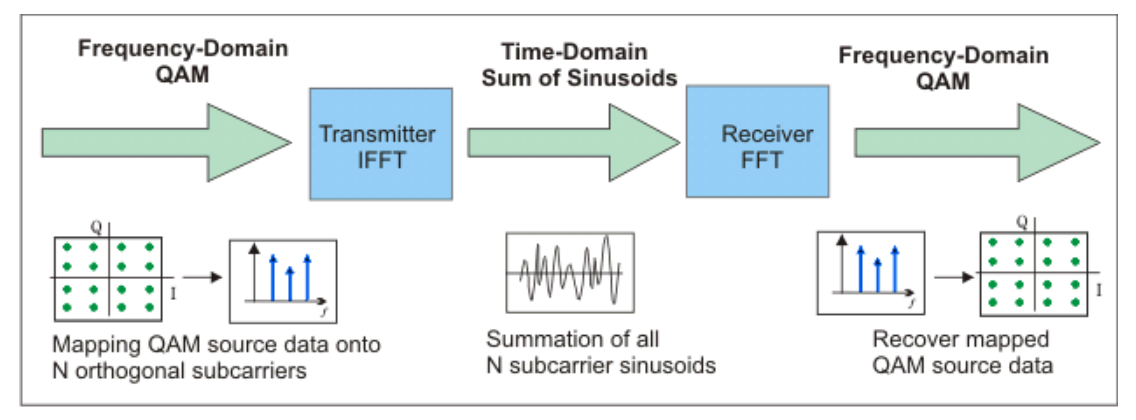
\includegraphics[width=1.0\textwidth]{./figure/chap 3/ofdm.png}
\caption{Block Diagram of Simplified OFDM  System}
\label{Fig 3.3}
\end{figure}

\subsection{MIMO}

Multiple-Input MIMO (Many-Input, Multiple-Output) is a wireless technology that uses multiple transmitters and receivers to carry more data at once. MIMO is supported by all 802.11n wireless equipment. The technology enables 802.11n to achieve faster rates than goods that do not have 802.11n.\cite{mimo}
MIMO must be supported by the station (mobile device) or the access point (AP) to be implemented. Both the station and the access point must support MIMO for the best performance and range.
Multipath, a natural radio-wave phenomenon, is used in MIMO technology. Multipath occurs when transmitted data bounces off walls, ceilings, and other obstacles, arriving at the receiving antenna numerous times at slightly varying angles and times. Multipath created interference and hindered wireless communications in the past. MIMO technology with multipath combines numerous, smart transmitters and receivers with an extra spatial dimension to improve performance and range.
By allowing antennas to mix data streams arriving from diverse paths and at different times, MIMO boosts the signal-capturing power of receivers. Smart antennas make use of spatial diversity technology, which makes use of unused antennas. When the number of antennas outnumbers the number of spatial streams, the antennas can boost receiver variety and range.\cite{CORVAJA2008288}

\begin{figure}[H]
\centering
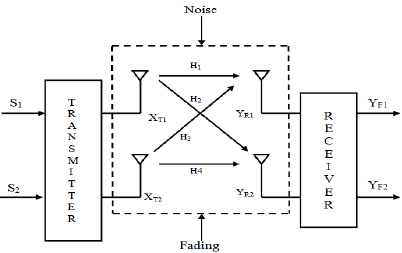
\includegraphics[width=1.0\textwidth]{./figure/chap 3/mimo.png}
\caption{Block Diagram of MIMO System}
\label{Fig 3.4}
\end{figure}


\section{Signals used for analysis}
Activity recognition using Wi-Fi data is not a completely new domain. Older methods of human activity recognition used Received Signal Strength Indication (RSSI) signal. But recently with the development in WLAN fields, newer standards starting from 802.11g can provide Channel State Information (CSI) signal too. In our proposed method, we utilized both signals to classify human activity more accurately. Here is an overview of these signals.

\subsection{RSSI}
The RSSI is a measurement of the signal's power at the moment it reaches the receiver. Signal energy diminishes with distance, according to signal propagation models and experiments. As a result, RSSI is frequently used in conjunction with multilateration algorithms to estimate position. When impediments are present in the region of interest, RSSI suffers from several drawbacks. RSSI values are distributed randomly and its correlation with the distance is not strong due to Multipath and shadowing fading effects. RSSI values are comparatively coarse information which is the result of averaging the amplitudes of all incoming signals to the receiver. These drawbacks lead to poor localization performance using RSSI \cite{Wang2016}. This problem can be solved by using rich channel information from different subcarriers.

\subsection{CSI}
In IEEE 802.11 a/g/n/ac/ax networks, data transmission and reception is done using OFDM. As discussed earlier, OFDM uses a number of orthogonal subcarriers to transmit data in multiple spatial paths. While a transmitting packet is in the medium, it is subjected to different obstructions, such as, fading, scattering and power loss. As the subcarriers follow different spatial paths, these obstructions affect each subcarrier differently. Thus this physical layer information specific to each subcarrier is known as Channel State Information (CSI). CSI is an overall depiction of the channel state that includes scattering, fading, and multipath effects in the signal's propagation. In contrast to the received power strength provided by RSSI, CSI statistics provide more information about the channel degradation effects that the signal suffers due to its granularity of sub-carrier frequencies and vector representation. Data is sent using MIMO and OFDM systems.

In narrow-band flat fading channel, a MIMO system is represented by:
\begin{equation}
    y_i = Hx_i + N_i
\end{equation}
where $y_i$ and $x_i$ are the received and the transmitted signal
vectors respectively, $H$ denotes the channel matrix which contains the CSI information and $N_i$ is the noise vector. To estimate the channel matrix $H$, a known training sequence or the pilot sequence is transmitted and channel response $H$ is measured at the receiver side. If the pilot sequence is expressed by $x_1, x_2, x_3, ... , x_n$, the received can be represented by: 
\begin{equation}
    Y = [y_1 + y_2 + ... + y_n] = HX + N
\end{equation}
Thus the channel matric can be determined by: 
\begin{equation}
    \hat{H} = \frac{Y}{X}
\end{equation}
For any MIMO system of $n \times m$ dimension, $H$ can be shown in matrix form:
\begin{equation}
    H_i = \begin{bmatrix}
    h_{11} & h_{12} & h_{13} & ... & h_{1m}\\ 
    h_{21} & h_{22} & h_{23} & ... & h_{2m}\\ 
    ... & ... & ... & ... & ... \\
    h_{n1} & h_{n2} & h_{n3} & ... & h_{nm}\\ 
    \end{bmatrix}
\end{equation}
where $i$ is the subcarrier index and $h_nm$ is a complex number representing the amplitude and phase information of Channel State Information (CSI).

\section{Machine Learning}
In the 1950s, a branch of artificial intelligence known as machine learning was discovered and developed. The earliest machine learning techniques date back to the 1950s, however there have been very few notable studies and advancements in this field. However, this field of study underwent a resurgence in the 1990s and has continued to this day. Future advancements in this field of study are expected. The complexity of analyzing and interpreting the data, which is continually expanding, is what has led to this development. The foundation of machine learning is the idea that, with the help of this growing data, the best model for the new data may be found among the old data. As a result, research into machine learning will continue along with the growth in data.\cite{mlArticle}
The actions performed by computers, which are based on an algorithm and follow specific procedures, have no margin for error. In some circumstances, computers make judgments based on the current sample data, which is different from commands that are created to produce an outcome depending on an input. In some circumstances, computers may err in their decision-making just like people do. Putting it another way, machine learning is the process of giving computers the capacity to learn from data and experience just like a human brain.\cite{jetol457046}The primary goal of machine learning is to develop models that can learn from previous data to become better, recognize complicated patterns, and find answers to new problems.\cite{Turk}

\subsection{Machine Learning Categories}
We can divide machine learning approaches in four categories.They are:
\begin{itemize}
    \item Supervised Learning
    \item Unsupervised Learning
    \item Semi-supervised Learning
    \item Reinforced Learning
\end{itemize}

Supervised learning is a technique where the currently available input data is used to arrive at the outcome set. Classification and regression supervised learning are the two categories of supervised learning.
\begin{enumerate}
    \item Classification: Dividing the data into the categories specified in the data set in accordance with their unique characteristics.
    \item Regression: Predicting or drawing conclusions about the other characteristics of the data from the known characteristics.
\end{enumerate}

Unsupervised learning is the technique where the output is not provided while training the model.The algorithms following this technique can be classified into two categories:
\begin{enumerate}
    \item Clustering: When intrinsic groupings in the data are unknown, finding groups of data that are comparable to one another.
    \item Association: Figuring out the links and relationships between the data in the same data collection.
\end{enumerate}

Semi-supervised learning is a method of machine learning that, during training, blends a sizable amount of unlabeled data with a small amount of labeled data. Between supervised learning (with labeled training data) and unsupervised learning is semi-supervised learning (with only labeled training data). It is a unique illustration of poor supervision. Either inductive learning or transductive learning may be referred to as semi-supervised learning.\cite{Zhu071contents}

Reinforcement learning is the challenge that an agent faces when learning behavior through trial-and-error interactions with a dynamic environment. Reinforcement learning differs from supervised learning in that it does not need the presentation of labeled input/output pairings or the explicit correction of suboptimal behaviors. Instead, the emphasis is on striking a balance between exploitation and exploration (of undiscovered territory) (of current knowledge). The benefits of supervised and RL algorithms can be combined with partially supervised RL algorithms.\cite{DBLP:journals/corr/cs-AI-9605103}

\section{Human Activity Recognition}
Human activity recognition is important for interpersonal interactions and human-to-human communication. It is challenging to extract since it contains details about a person's identity, personality, and psychological condition. One of the key research topics in the fields of computer vision and machine learning is the human capacity for activity recognition. This research has led to the need for multiple activity detection systems in numerous applications, such as video surveillance systems, human-computer interaction, and robotics for characterizing human behavior. Most of the work in human activity recognition assumes a figure-centric scene of an uncluttered background, where the actor is free to perform an activity. The development of a fully automated human activity recognition system, capable of classifying a person’s activities with low error, is a challenging task due to problems, such as background clutter, partial occlusion, changes in scale, viewpoint, lighting and appearance, and frame resolution.\cite{10.3389/frobt.2015.00028}

To solve these issues, a task is needed that combines three elements: (i) background subtraction, in which the system tries to distinguish between the foreground's changing or moving objects and the background's parts;\cite{1032799}\cite{s19061352} (ii) human tracking, in which the system tracks a person's motion over time;\cite{10.1016/j.patcog.2013.10.019} and (iii) human action and object detection, in which the system can localize a person's activity.\cite{Ganetal}

\begin{figure}[H]
\centering
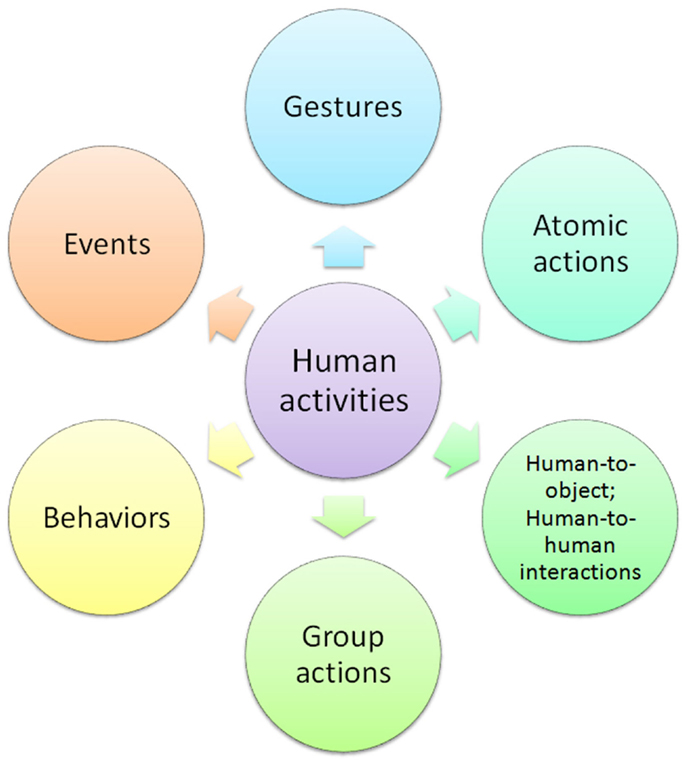
\includegraphics[width=0.7\textwidth]{./figure/chap 3/3.jpg}
\caption{Decomposition of human activities.}
\label{Fig 3.5}
\end{figure}

\section{Classification Algorithms}
Classification algorithm is a Supervised Learning technique that is used to categorize new observations based on training data. In classification, a program makes use of the dataset or observations that are provided to learn how to categorize new observations into various classes or groups. Some algorithms are discussed here:
\begin{itemize}
    \item SVM: Support vector machines (SVMs) are a group of supervised learning techniques for classifying data, performing regression analysis, and identifying outliers. Support vector machines have the following benefits: efficient in high-dimensional environments. Still useful in situations where the number of dimensions exceeds the number of samples.\cite{svm}
    \item Random Forest: A large number of decision trees are built during the training phase of the random forests or random decision forests ensemble learning approach, which is used for classification, regression, and other tasks. The class that the majority of the trees chose is the output of the random forest for classification problems. Decision trees tend to overfit their training set, and random decision forests correct for this. Although they frequently outperform decision trees, gradient boosted trees are more accurate than random forests.\cite{rforest}
    \item Extra Trees Classifier: In essence, it involves dividing a tree node while severely randomizing the choice of attribute and cut-point. In the worst situation, it creates completely random trees, whose architectures are independent of the learning sample's output values. By selecting the right parameter, the strength of the randomization can be adjusted to the particulars of the problem. The algorithm's biggest advantage, aside from accuracy, is computational speed.\cite{etclassifier}
        \begin{figure}[H]
        \centering
        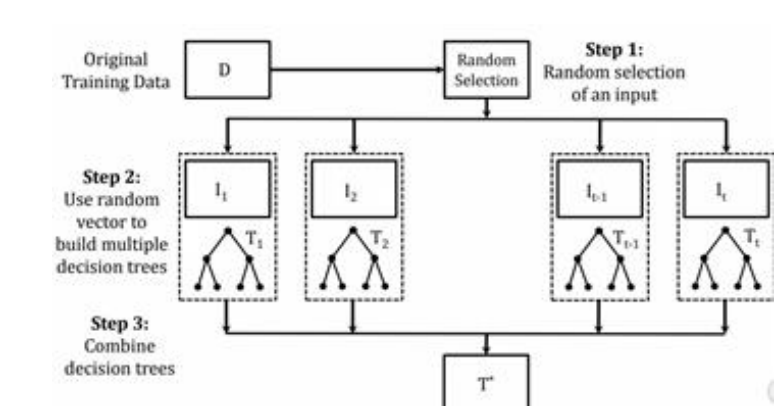
\includegraphics[width=0.7\textwidth]{./figure/chap 3/4.png}
        \caption{Visual Representation of Extra Trees Classifier.}
        \label{Fig 3.6}
        \end{figure}

    
    \item Artificial Neural Network(ANN): Artificial neural network is based on research into the brain and nervous system, as seen in Fig. 1. Although they employ a condensed set of biological brain system ideas, these networks mimic biological neural networks. Particularly, ANN models mimic the electrical activity of the nerve system and brain. Connected to other processing elements are processing elements (sometimes called neurodes or perceptrons). The neurodes are typically organized in layers or vectors, with the output of one layer acting as the input for the following layer and maybe other layers.\cite{ann}
        \begin{figure}[H]
        \centering
        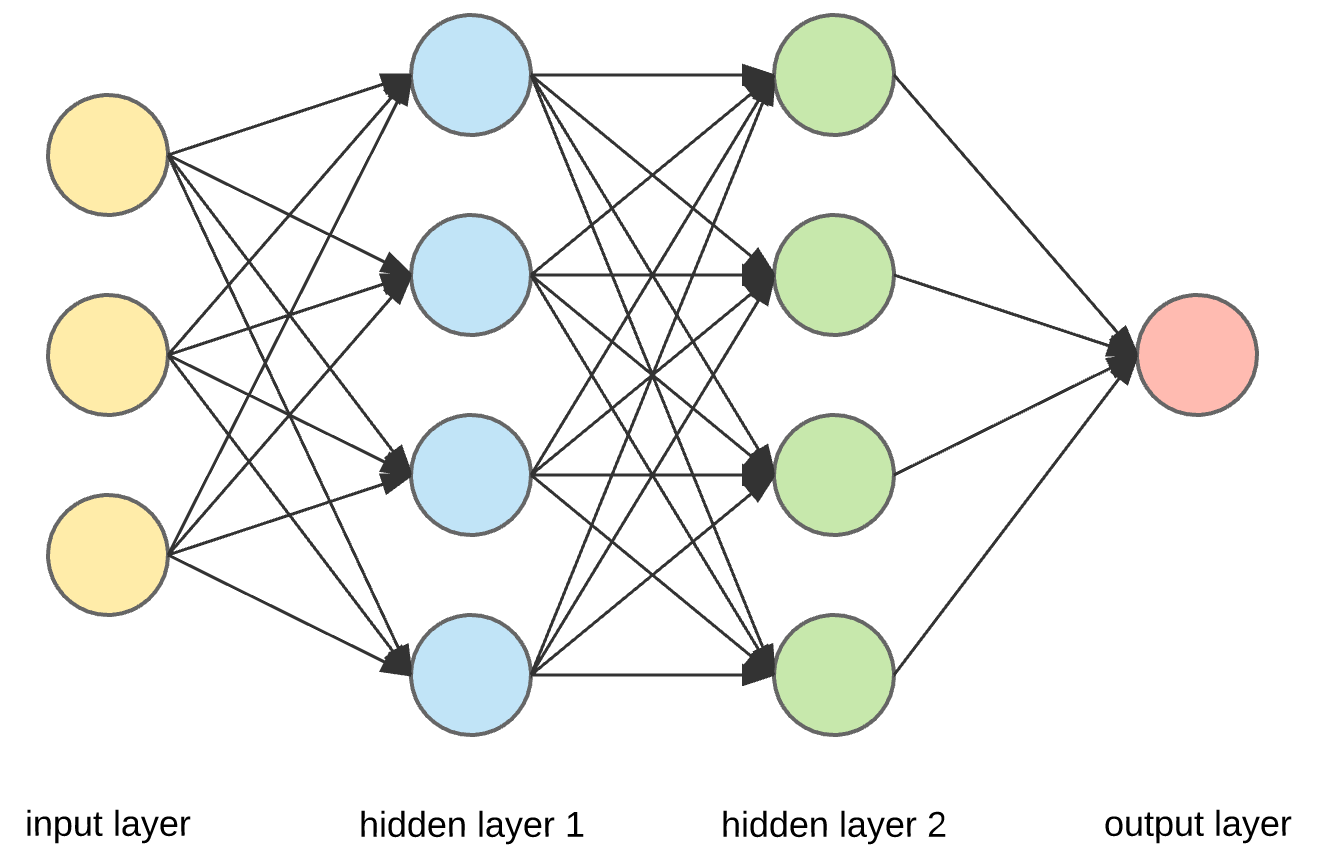
\includegraphics[width=0.7\textwidth]{./figure/chap 3/5.png}
        \caption{Visual Representation of an Artificial Neural Network.}
        \label{Fig 3.6}
        \end{figure}

\end{itemize}






